% @Author: Jacem Chaieb
% @Date:   2015-07-26 13:42:06
% @Last Modified by:   Jacem Chaieb
% @Last Modified time: 2016-04-12 15:37:31

%%%%%%%%%%%%%%%%%%%%%%%%%%%%%%%%%%%%%%%%%%%%%%%%%%%%%%%%%%%%%%%%%%%%%%%%%%%
% This is the main file
% You can add/remove chapters/pdf files here
%%%%%%%%%%%%%%%%%%%%%%%%%%%%%%%%%%%%%%%%%%%%%%%%%%%%%%%%%%%%%%%%%%%%%%%%%%%

\documentclass[12pt, oneside, a4paper]{enis-pfe-report}

%%%%%%%%%%%%%%%%%%%%%%%%%%%%%%%%%%%%%%%%%%%%%%%%%%%%%%%%%%%
% Define code variables
%%%%%%%%%%%%%%%%%%%%%%%%%%%%%%%%%%%%%%%%%%%%%%%%%%%%%%%%%%%
\graphicspath{{images/}}

%%%%%%%%%%%%%%%%%%%%%%%%%%%%%%%%%%%%%%%%%%%%%%%%%%%%%%%%%%%
%% Include required packages
%%%%%%%%%%%%%%%%%%%%%%%%%%%%%%%%%%%%%%%%%%%%%%%%%%%%%%%%%%%
%\usepackage{showframe}

\usepackage[skins]{tcolorbox}
\usepackage[francais,english]{babel}
\usepackage[english]{varioref}
\usepackage[export]{adjustbox}
\usepackage{acro}
\usepackage{setspace}
\usepackage{minted}
\usepackage{color}
\usepackage{tabularx}
\usepackage{ctable}
\usepackage{graphicx}
\usepackage{multirow}
\usepackage{tikz}
\usepackage{seqsplit}
\usepackage{fontenc}
%\usepackage{lipsum}
%\usepackage{todonotes}
\usepackage{wrapfig}
\usepackage{setspace}
\usepackage[all]{nowidow}

\usepackage[sorting=none, backend=bibtex]{biblatex}
\addbibresource{001-report}

%% TODO: Remove this function when done %%
\newcommand\todoin[2][]{\todo[inline, caption={2do}, #1]{
\begin{minipage}{\textwidth-4pt}#2\end{minipage}}}

%%%%%%%%%%%%%%%%%%%%%%%%%%%%%%%%%%%%%%%%%%%%%%%%%%%%%%%%%%%
% Include useful commands
%%%%%%%%%%%%%%%%%%%%%%%%%%%%%%%%%%%%%%%%%%%%%%%%%%%%%%%%%%%
% @Author: Jacem Chaieb
% @Date:   2015-07-26 13:42:06
% @Last Modified by:   Jacem Chaieb
% @Last Modified time: 2016-04-12 15:42:00

%%%%%%%%%%%%%%%%%%%%%%%%%%%%%%%%%%%%%%%%%%%%%%%%%%%%%%%%%%%%%%%%%%%%%%%%%%%
% In this file, you will put the details of your graduation project
%%%%%%%%%%%%%%%%%%%%%%%%%%%%%%%%%%%%%%%%%%%%%%%%%%%%%%%%%%%%%%%%%%%%%%%%%%%

\newcommand{\reportTitle} {%
  \textsc{Graduation Project}%
}

\newcommand{\reportAuthor} {%
  FirstName \textsc{LastName}%
}

\newcommand{\reportSubject} {%
  My very attractive \\ Title%
}

\newcommand{\dateSoutenance} {%
  12/12/1234%
}

\newcommand{\studyDepartment} {%
  Computer Engineering \& Applied Mathematics Department%
}

\newcommand{\ENIS} {%
  National Engineering School of Sfax%
}

\newcommand{\codePFE} {% Reference
  DIMA-033%
}

\newcommand{\juryPresident} {%
  Mr Foulen \textsc{Fouleni}%
}
\newcommand{\juryPresidentDesc} {%
  President%
}

\newcommand{\juryMemberOne} {%
  Ms Foulena \textsc{Foulenia}%
}
\newcommand{\juryMemberOneDesc} {%
  Supervisor %Mentor
}

\newcommand{\juryMemberTwo} {%
  Mr Foulen \textsc{Fouleni}%
}
\newcommand{\juryMemberTwoDesc} {%
  Reviewer% Examiner, Reporter
}

\newcommand{\specialcell}[1]{%
  \begin{tabularx}{\textwidth}{@{}X@{}}#1\end{tabularx}%
}

%%%%%%%%%%%%%%%%%%%%%%%%%%%%%%%%%%%%%%%%%%%%%%%%%%%%%%%
% Add your own commands here
%%%%%%%%%%%%%%%%%%%%%%%%%%%%%%%%%%%%%%%%%%%%%%%%%%%%%%%
\newcommand{\MyCommand} {%
  Does nothing really%
}

%%%%%%%%%%%%%%%%%%%%%%%%%%%%%%%%%%%%%%%%%%%%%%%%%%%%%%%
% Add your own acronyms here
%%%%%%%%%%%%%%%%%%%%%%%%%%%%%%%%%%%%%%%%%%%%%%%%%%%%%%%
\DeclareAcronym{ENIS}{%
  short=ENIS,%
  long=National Schoole of Engineering of Sfax%
}

\hypersetup{
  pdftitle={\reportTitle~-~\reportSubject},%
  pdfauthor={\reportAuthor},%
  pdfsubject={\reportSubject},%
  pdfkeywords={report} {internship} {pfe} {enis}
}

\begin{document}
  \begin{pfe-enis}
    \pagenumbering{roman}% i ii iii iv ...

    % \listoftodos{}

    % Front matter
    % @Author: Jacem Chaieb
% @Date:   2015-07-26 13:42:06
% @Last Modified by:   Jacem Chaieb
% @Last Modified time: 2016-04-12 15:23:40

%%%%%%%%%%%%%%%%%%%%%%%%%%%%%%%%%%%%%%%%%%%%%%%
% Only edit this file for fine tuning to your own needs/liking
% There isn't really much to edit here
%%%%%%%%%%%%%%%%%%%%%%%%%%%%%%%%%%%%%%%%%%%%%%%

\thispagestyle{empty}
\begin{titlepage}
\begin{center}

%%%%%%%%%%%%%%%%%%%%%%%%%%%%%%%%%%%%%%%%%%%%%%%
% THE HEADER
%%%%%%%%%%%%%%%%%%%%%%%%%%%%%%%%%%%%%%%%%%%%%%%
{%
  \fontsize{9pt}{9pt}\selectfont%
  \begin{tabularx}{\textwidth}{ @{} p{0.4\textwidth} @{} m{0.2\textwidth} @{} p{0.4\textwidth} @{} }
    %
    %
    %
    % Line 1
    \centering%
    Republic of Tunisia\\%
    Ministry of Higher Education, Scientific Research %
    and Information and Communication Technologies\\%
    &%
    % Column 2
    \centering%
    \multirow{2}{\linewidth}{%
      \centering%
      
\includegraphics[width=2.5cm, height=2.5cm]{logo-enis.pdf}%
    }%
    &%
    % Column 3
    \centering%
    \studyDepartment%
    % Engineering Education Computer Engineering and Applied Mathematics Discipline%
    % Cycle de Formation d'Ingénieurs dans la Discipline Génie \studyDepartment%
    \tabularnewline%
    %
    %
    %
    % Line 2
    \centering%
    %\rule{2cm}{0.75pt}\\
    Sfax University\\
    \ENIS{}
    &%
    % Column 2 is empty (contains the ENIS logo)
    &%
    % Column 3
    \centering%
    \textbf{%
    ST-EN07/00\\%
    \reportTitle{}\\%
    Serial N°: 2015 / \codePFE%
    }
    \tabularnewline%
    \arrayrulecolor{reportType}%
    \specialrule{0.75pt}{2pt}{0pt}%
    \specialrule{2.00pt}{1pt}{0pt}%
  \end{tabularx}
}


%%%%%%%%%%%%%%%%%%%%%%%%%%%%%%%%%%%%%%%%%%%%%%%
% THE PAGE CONTENT
%%%%%%%%%%%%%%%%%%%%%%%%%%%%%%%%%%%%%%%%%%%%%%%

\vspace{30pt} {%
  \renewcommand*{\familydefault}{\defaultFont}
  \fontsize{46pt}{46pt}\selectfont%
  % MEMOIRE\\%
  \reportTitle{}\\\textsc{Report}\\%
}

\vspace{30pt}%
\textbf{\textit{presented at}}\\

\vspace{10pt}
\ENIS{}\\
(\studyDepartment)\\

\vspace{30pt}
\textbf{\textit{in order to obtain the}}\\

\vspace{10pt}
National Engineering Diploma in Computer Science\\
%du Diplôme National d'Ingénieur en Génie \studyDepartment\\

\vspace{30pt}
\textbf{\textit{by}}\\
\vspace{10pt} {%
  \fontsize{18pt}{18pt}\selectfont%
  \textbf{\reportAuthor}\\
}%

\vspace{10pt} {%
  \renewcommand*{\familydefault}{\defaultFont}
  \fontsize{27pt}{27pt}\selectfont%
  \HRule%
  \vspace{10pt}
  \reportSubject{}\\%
  \vspace{10pt}
  \HRule%
}

\vspace{10pt}
Defended on~\dateSoutenance~in front of the committee composed of\\
%Soutenu le \dateSoutenance, devant la commission d'examen:\\
\vspace{20pt}
\begin{tabular}{p{0.3\linewidth} p{0.15\linewidth}}
  \juryPresident{} & \juryPresidentDesc{}\\
  \juryMemberOne{} & \juryMemberOneDesc{}\\
  \juryMemberTwo{} & \juryMemberTwoDesc{}\\
\end{tabular}

\vfill

\end{center}
\end{titlepage}
    \cleardoublepage%

    % @Author: Jacem Chaieb
% @Date:   2015-07-26 13:42:06
% @Last Modified by:   Jacem Chaieb
% @Last Modified time: 2016-04-12 15:43:36

\chapter*{Dedication}
\addcontentsline{toc}{chapter}{Dedication}
\thispagestyle{empty}
%
%For all they have endured to satisfy all my needs and wishes
\begin{center}
  Put your dedication lines here ~\\
  And try to be expressive ;) ~\\


  Lorem ipsum dolor sit amet, consectetur adipisicing elit, sed do eiusmod ~\\
  tempor incididunt ut labore et dolore magna aliqua. Ut enim ad minim veniam, ~\\
  quis nostrud exercitation ullamco laboris nisi ut aliquip ex ea commodo ~\\
  consequat. Duis aute irure dolor in reprehenderit in voluptate velit esse ~\\
  cillum dolore eu fugiat nulla pariatur. Excepteur sint occaecat cupidatat non ~\\
  proident, sunt in culpa qui officia deserunt mollit anim id est laborum ~\\
\end{center}
%
\nopagebreak{%
  % And maybe a quote here
  \raggedright\hspace{5.75cm} To all of you,~\\
  \raggedright\hspace{7.75cm} I dedicate this work\@.~\\~\\~\\
  %
  \raggedleft\normalfont\large\itshape{} \reportAuthor\par%
}
%
%
%
%
%
%
\cleardoublepage%
\chapter*{Thanks}
\addcontentsline{toc}{chapter}{Thanks}
\thispagestyle{empty}
%
And put your thanks here. ~\\

Lorem ipsum dolor sit amet, consectetur adipisicing elit, sed do eiusmod
tempor incididunt ut labore et dolore magna aliqua. Ut enim ad minim veniam,
quis nostrud exercitation ullamco laboris nisi ut aliquip ex ea commodo
consequat. Duis aute irure dolor in reprehenderit in voluptate velit esse
cillum dolore eu fugiat nulla pariatur. Excepteur sint occaecat cupidatat non
proident, sunt in culpa qui officia deserunt mollit anim id est laborum. Lorem ipsum dolor sit amet, consectetur adipisicing elit, sed do eiusmod
tempor incididunt ut labore et dolore magna aliqua. Ut enim ad minim veniam,
quis nostrud exercitation ullamco laboris nisi ut aliquip ex ea commodo
consequat. Duis aute irure dolor in reprehenderit in voluptate velit esse
cillum dolore eu fugiat nulla pariatur. Excepteur sint occaecat cupidatat non
proident, sunt in culpa qui officia deserunt mollit anim id est laborum.
    \cleardoublepage%

    \tableofcontents
    \addcontentsline{toc}{chapter}{\contentsname}
    \cleardoublepage%

    \listoffigures
    \addcontentsline{toc}{chapter}{\listfigurename}
    \cleardoublepage%

    % \listoftables
    % \addcontentsline{toc}{chapter}{\listtablename}
    % \cleardoublepage

    %\printglossary[type=\acronymtype, title=Abbreviations]
    \printacronyms[header=chapter*, name=Acronyms]
    \addcontentsline{toc}{chapter}{Acronyms}
    \cleardoublepage%

    \sloppy

    \pagenumbering{arabic}% 1 2 3 4 5
    \doublespacing{}% Double spacing between lines

    \addtocontents{toc}{\protect\setcounter{tocdepth}{2}}

    % Main matter
    % @Author: Jacem Chaieb
% @Date:   2015-07-26 13:42:06
% @Last Modified by:   Jacem Chaieb
% @Last Modified time: 2016-04-12 15:49:40

%%%%%%%%%%%%%%%%%%%%%%%%%%%%
% CHAPTER                  %
%%%%%%%%%%%%%%%%%%%%%%%%%%%%
\chapter*{Introduction}
\label{chap:general_intorduction}
\markboth{\MakeUppercase{Introduction}}{}%
\addcontentsline{toc}{chapter}{Introduction}%

Welcome to \Ac{ENIS}. ~\\
Again, welcome to \Ac{ENIS}. ~\\
Your introduction goes here. ~\\

Lorem ipsum dolor sit amet, consectetur adipisicing elit, sed do eiusmod
tempor incididunt ut labore et dolore magna aliqua. Ut enim ad minim veniam,
quis nostrud exercitation ullamco laboris nisi ut aliquip ex ea commodo
consequat. Duis aute irure dolor in reprehenderit in voluptate velit esse
cillum dolore eu fugiat nulla pariatur. Excepteur sint occaecat cupidatat non
proident, sunt in culpa qui officia deserunt mollit anim id est laborum.
Lorem ipsum dolor sit amet, consectetur adipisicing elit, sed do eiusmod
tempor incididunt ut labore et dolore magna aliqua. Ut enim ad minim veniam,
quis nostrud exercitation ullamco laboris nisi ut aliquip ex ea commodo
consequat. Duis aute irure dolor in reprehenderit in voluptate velit esse
cillum dolore eu fugiat nulla pariatur. Excepteur sint occaecat cupidatat non
proident, sunt in culpa qui officia deserunt mollit anim id est laborum.
    \cleardoublepage%

    % @Author: Jacem Chaieb
% @Date:   2015-07-26 13:42:06
% @Last Modified by:   Jacem Chaieb
% @Last Modified time: 2016-04-12 15:45:38

%%%%%%%%%%%%%%%%%%%%%%%%%%%%
% CHAPTER                  %
%%%%%%%%%%%%%%%%%%%%%%%%%%%%
\chapter{Chapter One}%
\label{chap:chapter_one}

%%%%%%%%%%%%%%%%%%%%%%%%%%%%
% SECTION                  %
%%%%%%%%%%%%%%%%%%%%%%%%%%%%
\section{Section One}
\label{chap:section_one}

  %%%%%%%%%%%%%%%%%%%%%%%%%%%%
  % SUBSECTION               %
  %%%%%%%%%%%%%%%%%%%%%%%%%%%%
  \subsection{Sub section One}

  And your chapter one goes here\cite{web001}\@. ~\\
  Lorem ipsum dolor sit amet, consectetur adipisicing elit, sed do eiusmod
  tempor incididunt ut labore et dolore magna aliqua. Ut enim ad minim veniam,
  quis nostrud exercitation ullamco laboris nisi ut aliquip ex ea commodo
  consequat. Duis aute irure dolor in reprehenderit in voluptate velit esse
  cillum dolore eu fugiat nulla pariatur. Excepteur sint occaecat cupidatat non
  proident, sunt in culpa qui officia deserunt mollit anim id est laborum.

  \begin{figure}[H]%
    \center%
    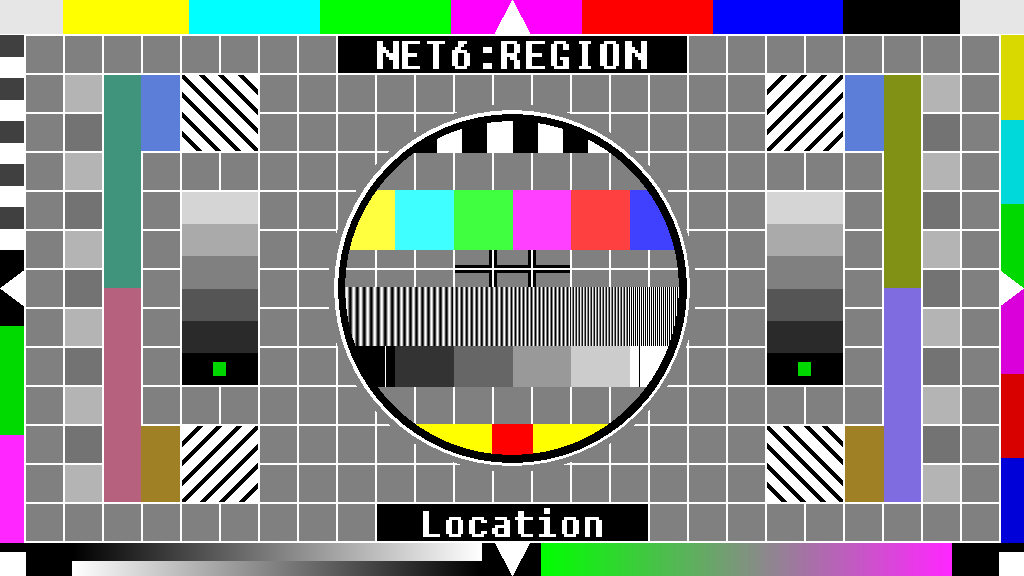
\includegraphics[width=0.3\textwidth]{test.png}%
    \caption[This is a test image]{Test Image}\label{fig:test}%
  \end{figure}

  %%%%%%%%%%%%%%%%%%%%%%%%%%%%
  % SUBSECTION               %
  %%%%%%%%%%%%%%%%%%%%%%%%%%%%
  \subsection{Sub section Two}

  This is a second subsection\cite{bazerman1988shaping}. ~\\
  Lorem ipsum dolor sit amet, consectetur adipisicing elit, sed do eiusmod
  tempor incididunt ut labore et dolore magna aliqua. Ut enim ad minim veniam,
  quis nostrud exercitation ullamco laboris nisi ut aliquip ex ea commodo
  consequat. Duis aute irure dolor in reprehenderit in voluptate velit esse
  cillum dolore eu fugiat nulla pariatur. Excepteur sint occaecat cupidatat non
  proident, sunt in culpa qui officia deserunt mollit anim id est laborum.

  \begin{description}\addtolength{\itemsep}{-0.35\baselineskip}%
    \item[\textbullet~\bfseries Menu Item] \hfill \\%
      Menu Description.~\\%
      {\textbf{Focus topics:~}\emph{Topic one, topic two, topic three, ...}}%
    %
    \item[\textbullet~\bfseries Menu Item] \hfill \\%
      Menu Description.~\\%
      {\textbf{Focus topics:~}\emph{Topic one, topic two, topic three, ...}}%
    %
    \item[\textbullet~\bfseries Menu Item] \hfill \\%
      Menu Description.~\\%
      {\textbf{Focus topics:~}\emph{Topic one, topic two, topic three, ...}}%
  \end{description}

  Also bullets such as:%
  \begin{itemize}\addtolength{\itemsep}{-0.35\baselineskip}%
    \item One%
    \item Two%
    \item Three%
    \item Four%
    \item \ldots%
  \end{itemize}%
  %

  And for more chaptes, just copy the file ``004-chapter1.tex'' and edit the content, and then you'll have to add it to ``001-report.tex''.
%%%%%%%%%%%%%%%%%%%%%%%%%%%%%%%%%%%%%%%%%%%%%%%%%%%%%%%%%%%%%%%%%%%%%%%%%%%%%%%%%%%%%%%%%%%%%%%%%%%%%%%%%%%%%%%%%%
    \cleardoublepage%

    % \include{004-chapter2}
    % \cleardoublepage%

    % \include{004-chapter3}
    % \cleardoublepage%

    % Back matter
    % @Author: Jacem Chaieb
% @Date:   2015-07-26 13:42:06
% @Last Modified by:   Jacem Chaieb
% @Last Modified time: 2016-04-12 15:45:56

\chapter*{Conclusion}
\label{chap:conclusion}
\markboth{\MakeUppercase{Conclusion}}{}%
\addcontentsline{toc}{chapter}{Conclusion}
  And a very interesting conclusion here\@. ~\\
  Lorem ipsum dolor sit amet, consectetur adipisicing elit, sed do eiusmod
  tempor incididunt ut labore et dolore magna aliqua. Ut enim ad minim veniam,
  quis nostrud exercitation ullamco laboris nisi ut aliquip ex ea commodo
  consequat. Duis aute irure dolor in reprehenderit in voluptate velit esse
  cillum dolore eu fugiat nulla pariatur. Excepteur sint occaecat cupidatat non
  proident, sunt in culpa qui officia deserunt mollit anim id est laborum.
  Lorem ipsum dolor sit amet, consectetur adipisicing elit, sed do eiusmod
  tempor incididunt ut labore et dolore magna aliqua. Ut enim ad minim veniam,
  quis nostrud exercitation ullamco laboris nisi ut aliquip ex ea commodo
  consequat. Duis aute irure dolor in reprehenderit in voluptate velit esse
  cillum dolore eu fugiat nulla pariatur. Excepteur sint occaecat cupidatat non
  proident, sunt in culpa qui officia deserunt mollit anim id est laborum.
    \cleardoublepage%

    % @Author: Jacem Chaieb
% @Date:   2015-11-28 03:20:19
% @Last Modified by:   Jacem Chaieb
% @Last Modified time: 2016-04-12 15:46:04

\chapter*{Appendix}
\label{chap:appendix}
\markboth{\MakeUppercase{Appendix}}{}
\addcontentsline{toc}{chapter}{Appendix}

  An appedix if you need it. ~\\

  Lorem ipsum dolor sit amet, consectetur adipisicing elit, sed do eiusmod
  tempor incididunt ut labore et dolore magna aliqua. Ut enim ad minim veniam,
  quis nostrud exercitation ullamco laboris nisi ut aliquip ex ea commodo
  consequat. Duis aute irure dolor in reprehenderit in voluptate velit esse
  cillum dolore eu fugiat nulla pariatur. Excepteur sint occaecat cupidatat non
  proident, sunt in culpa qui officia deserunt mollit anim id est laborum.
  Lorem ipsum dolor sit amet, consectetur adipisicing elit, sed do eiusmod
  tempor incididunt ut labore et dolore magna aliqua. Ut enim ad minim veniam,
  quis nostrud exercitation ullamco laboris nisi ut aliquip ex ea commodo
  consequat. Duis aute irure dolor in reprehenderit in voluptate velit esse
  cillum dolore eu fugiat nulla pariatur. Excepteur sint occaecat cupidatat non
  proident, sunt in culpa qui officia deserunt mollit anim id est laborum.
    \cleardoublepage%

    % @Author: Jacem Chaieb
% @Date:   2015-07-26 13:42:06
% @Last Modified by:   Jacem Chaieb
% @Last Modified time: 2016-04-12 15:35:09

%%%%%%%%%%%%%%%%%%%%%%%%%%%%%%%%%%%%%%%%%%%%%%%%%%%%
% Don't touch this, it is auto generated
%%%%%%%%%%%%%%%%%%%%%%%%%%%%%%%%%%%%%%%%%%%%%%%%%%%%
\nocite{*}

\phantomsection{}
\addcontentsline{toc}{chapter}{Webography}
\printbibliography[title={Webography},type=online]

\phantomsection{}
\addcontentsline{toc}{chapter}{Bibliography}
\printbibliography[title={Bibliography},nottype=online]

    \cleardoublepage%

    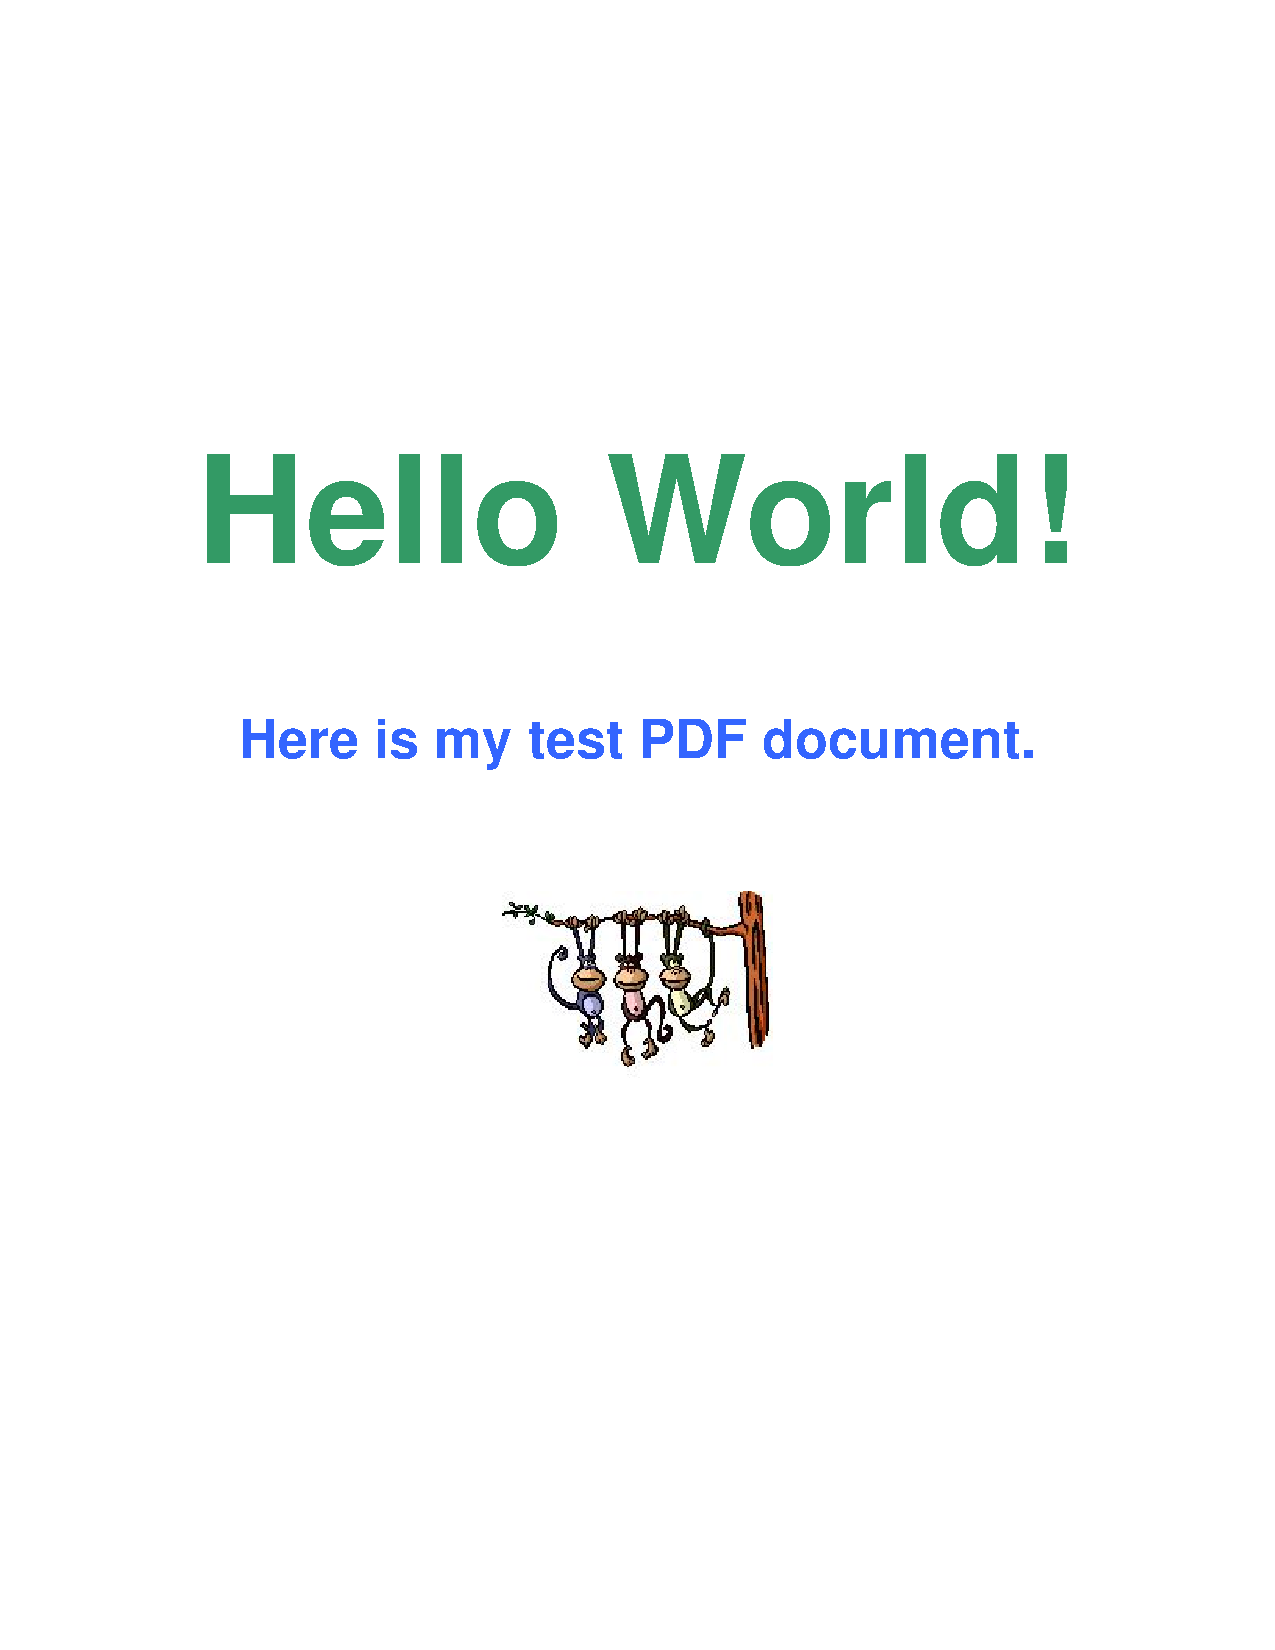
\includepdf[pages={-}]{008-abstract.pdf}
    %\include{008-abstract}
    \cleardoublepage%

    \addtocontents{toc}{\protect\setcounter{tocdepth}{3}}

  \end{pfe-enis}
\end{document}